\section{Threaded elements and screws}
	\begin{SCfigure}[2][b]
		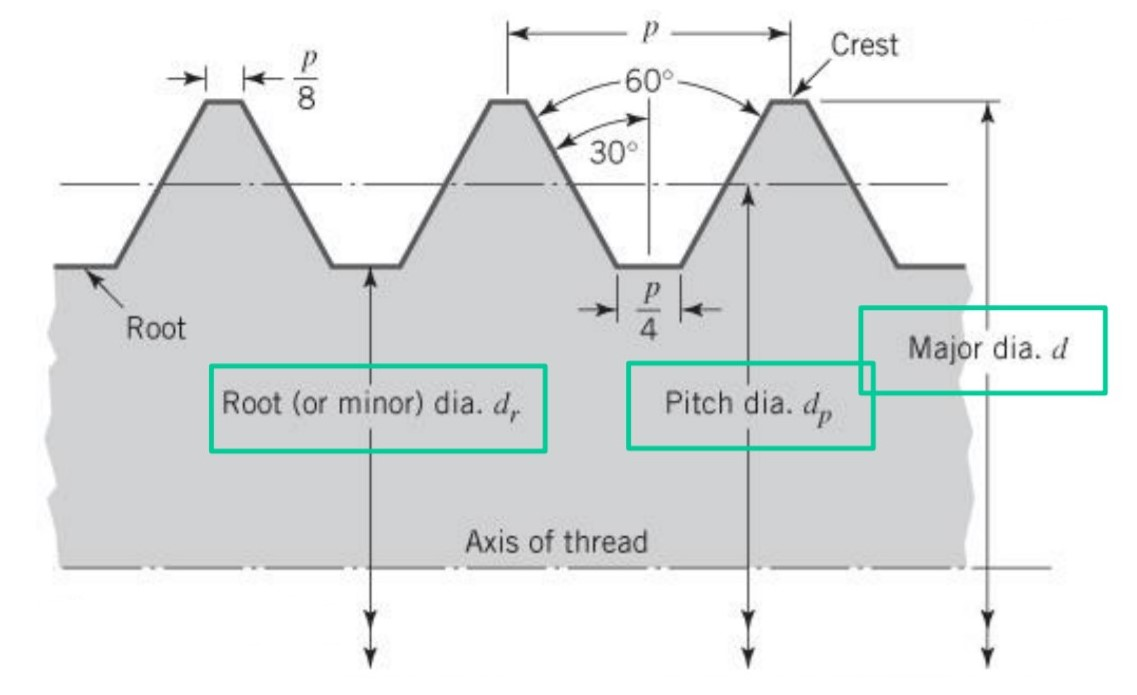
\includegraphics[width=0.5\linewidth]{thread-profile} 
		\caption{cross section of a threaded element such a screw.} \label{fig:screwsection}
	\end{SCfigure}
	
	Starting with the drawing in figure \ref{fig:screwsection}, we can see that the main elements of a threaded component are
	\begin{multicols}{2}
	\begin{itemize}
		\item the \textbf{root} (inner) diameter $d_r$;
		\item the \textbf{major/nominal} diameter $d$ measured on the outer \textit{ring} of the screw;
		\item the \textbf{pitch} diameter $d_p$ measured at half of the thread;
		\item the axial \textbf{pitch} $p$ (\textit{passo}) as the distance between contiguous thread;
		\item a \textbf{lead} $L$, describing the travel of a single pitch for a pitch round;
		\item the \textbf{helix angle} $\lambda$ such that $L=\pi d_p \tan \lambda$;
		\item for some elements important is the \textbf{\textit{inclination}} $\alpha$ of the thread that's typically $30^\circ$.
	\end{itemize}
	\end{multicols}

	In general each standard has it's own way to describe the profile of the threads. Each screw should be described by a nominal diameter (12), a length of the screw (50), a reference standard (\texttt{ISO 4014}) and a property class (8.8) as in the following case:
	\begin{center}
		screw \texttt{ M12 x 50 ISO 4014-8.8 }
	\end{center}
	
	According to ISO definitions the first number of the property class represent the minimum tensile strength multiplied by $100 MPa$, while the second is the relative value of the yielding strength; for the example before the property class \texttt{ISO 4014-8.8} means having a screw with ultimate tensile strength $\suts \geq 8\cdot 100 MPa$ and a yield of $\sys \geq 0.8 \suts = 640MPa$. In table \ref{tab:classproperty} a set of possible property classes have been reported. Tables \ref{tab:bolts} and \ref{tab:boltsdim} reports dimension for the \texttt{ISO} metric screws.
	
	\begin{table}[bht]
		\centering
		\rule{0.9\linewidth}{1pt}
		\caption{yield strength $\sys$ and ultimate tensile strength $\suts$ for different classes of bolts according to \texttt{ISO 4014} with related allowed nominal diameter and nut class.}
		\label{tab:classproperty}		
		\begin{tabular}{c | c c c | c }
			\texttt{ISO-4014} class & $d_{nom}$ & $\sys$ (min) & $\suts$ (min) & nut class \\ \hline
			4.6 & 5-100 & 240 & 400 \\
			4.8 & 1.6-16 & 340 & 420 \\
			5.8 & 5-24 & 420 & 520 & 5\\ \hdashline
			8.8 & \multirow{3}{*}{17-72} & \multirow{3}{*}{660} & \multirow{3}{*}{830} & \multirow{3}{*}{8} \\
			8.8 low carbon & & & \\
			8.8.3 & & & \\  \hdashline
			10.9 & \multirow{3}{*}{5-100} & \multirow{3}{*}{940} & \multirow{3}{*}{1040} & \multirow{3}{*}{10} \\
			10.9 low carbon & & & \\
			10.9.3 & & & \\  \hdashline
			12.9 & 1.6-100 & 1100 & 1220 & 12
		\end{tabular}
		\rule{0.9\linewidth}{1pt}
	\end{table}
	
	\begin{table}[p]
		\centering
		\rule{0.9\linewidth}{1pt}
		\caption{ \texttt{ISO} metric threads.}
		\label{tab:bolts}		
		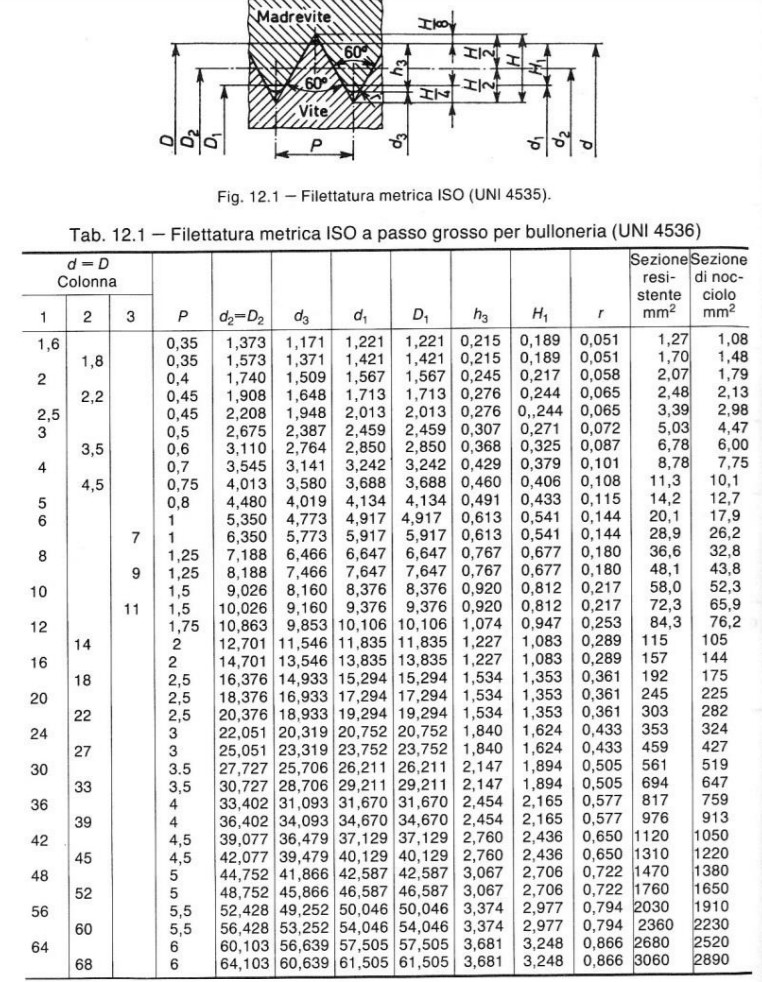
\includegraphics[width=0.9\linewidth]{metricscrews}
		\rule{0.9\linewidth}{1pt}
	\end{table}
	\begin{table}[p]
		\centering
		\rule{0.9\linewidth}{1pt}
		\caption{ \texttt{ISO} metric threads geometrical parameters.}
		\label{tab:boltsdim}		
		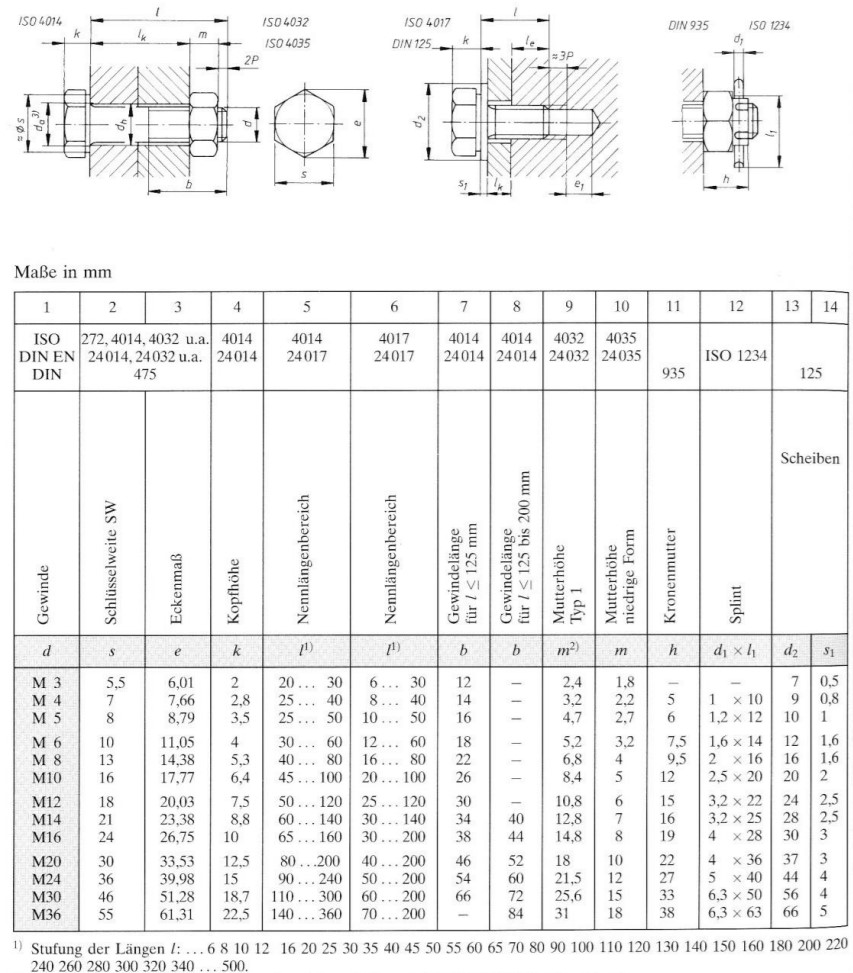
\includegraphics[width=0.9\linewidth]{bolt-dims}
		\rule{0.9\linewidth}{1pt}
	\end{table}

	
\subsection{Power screws}
	Power screws (figure \ref{fig:powerscrew}) use mechanical advantage of the threaded element in order to lift weights.
	\begin{SCfigure}[3][b!]
		\centering 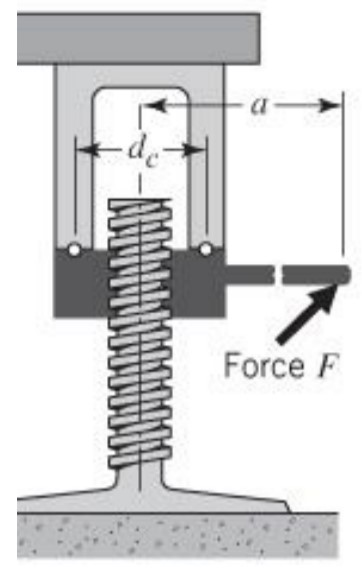
\includegraphics[width=3cm]{power-screw} 
		\caption{example of a power screw and representation of the main geometric dimension and loads.} \label{fig:powerscrew}
	\end{SCfigure}
	
	By doing a a force equilibrium it's possible to compute the torque $T$ (determined by the applied force $F$, hence $T = Fa$) that has to be transmitted in order to lift a weight $w$ depending from the friction coefficient $f$ between screw and collar and the friction coefficient $f_c$ between the collar (of diameter $d_c$) and the support of the weight to be lifted:
	\begin{equation}
		T = \frac{w d_m}{2} \frac{f\pi d_m + \cos\alpha_n L}{-fL + \pi d_m \cos\alpha_n} + \frac{wf_cd_c}{2}
	\end{equation}
	Power screws can be mainly of two types: \textbf{self locking} if, with no torque applied, the system stay locked due to the friction contact between the thread and the lever, while if the system (over no force applied) moves then it's referred as \textbf{overhauling screw}. The condition to have a self locking screw is
	\[ \textrm{if } f \geq \frac{L \cos \alpha_n}{\pi d_m} = \tan \lambda \cos \alpha_n \qquad \Rightarrow \quad \textrm{self-locking screw} \]
	Power screws are subjected to an \textbf{efficiency} $e$ (ratio between output and input power in the system) that's lowered by the dissipation due to friction and that's equal to
	\[ e = \frac{\cos \alpha_n - f \tan \lambda}{\cos \alpha_n + f \cot \lambda} \]
	
	
\subsection{Tensile bolted connection verification}
	In the case of a tensile bolted joint we can model both the screw and the members as springs (whose stiffness has to be computed independently) that are congruent, so such that the displacement $\Delta l_b$ of the bolts relates to the one of the member $\Delta l_f$ is a way such that the interference $i$ is
	\[ i = \Delta l_b - \Delta l_f \]		
	This interference can then be used to compute the preload of the bolted connection in the verification of the system.
	
	\begin{SCfigure}[2][bht]
		\centering 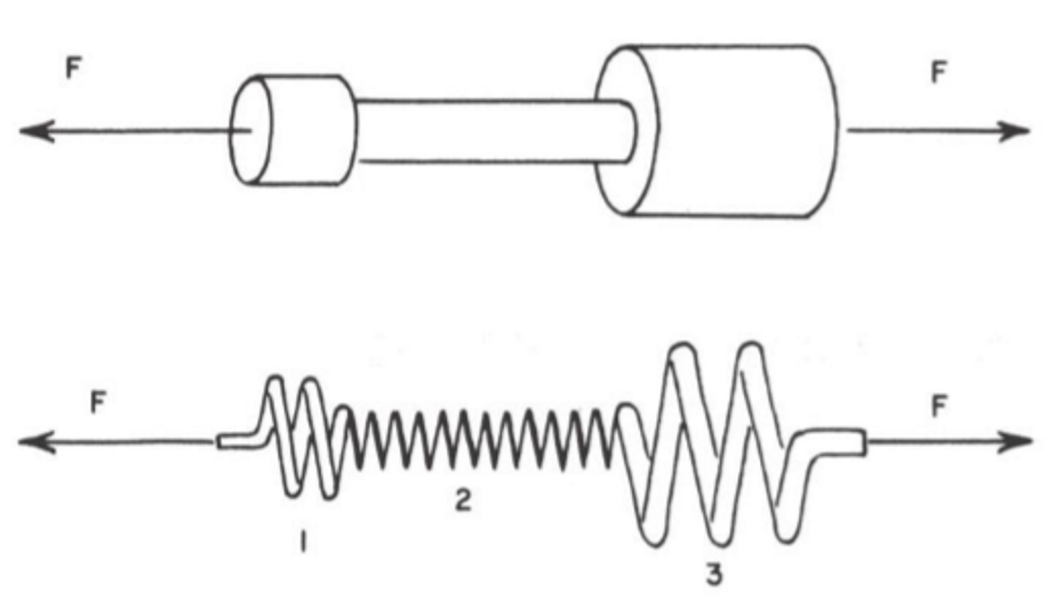
\includegraphics[width=5cm]{keq}
		\caption{example of a beam and it's spring model; the springs are connected in series with elastic modulus depending on the property of the sections.} \label{fig:keq}
	\end{SCfigure}

	\paragraph{Bolts} The bolts (but similarly the members) can be modelled as a series of springs connected in series whose equivalent stiffness $K_b$ is computed as
	\begin{equation} \label{eq:springseries}
		K_b = \left( \sum_i \frac{l_i}{E A_i} \right)^{-1}
	\end{equation}
	In a bolted connection the screw elongates in order to increase the pushing force tightening the components, and so the tensile force $F$ applied by the screw is equal to $K_b \, \Delta l_b$.
	
	\paragraph{Members} Considering the members, the equivalent stiffness is harder to compute, however experimental analysis determined that the distribution of the stress due to the tensile load can be described as a cone with an inclination $\alpha$ typically of $30^\circ$ (as in figure \ref{fig:memberstiff})	.
	
	By integration of the equivalent stiffness of each infinitesimal hollow cone it's possible to compute each member's stiffness as
	\begin{equation} \label{eq:conicalstiffness}
		K_i = \frac{\pi E d \tan \alpha}{\ln \left( \frac{D-d}{D+d} \frac{d_0+d}{d_0-d} \right)}
	\end{equation}
	As for the bolt, the equivalent stiffness $K_f$ of the member can be computed considering the springs placed in series (equation \ref{eq:springseries}).
	\begin{figure}[bht]
		\centering
		\begin{subfigure}{0.48\linewidth}
			\centering 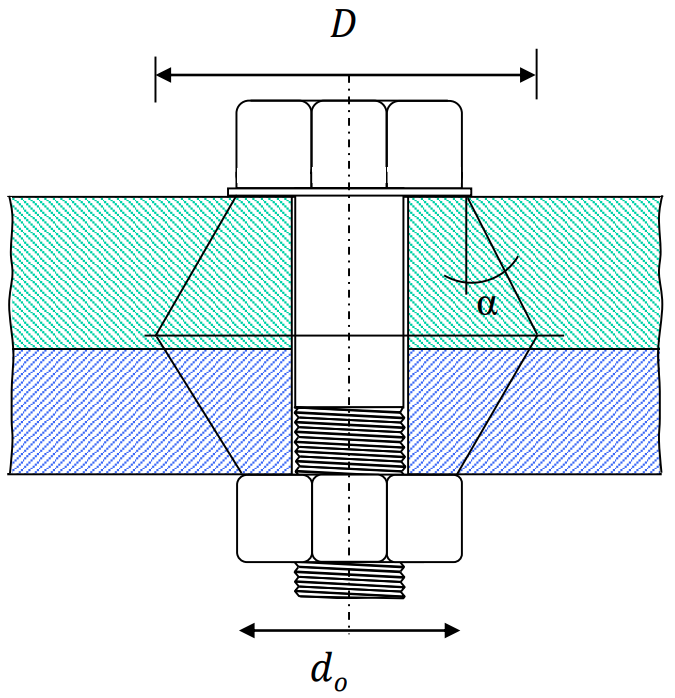
\includegraphics[width=4cm]{membstiff} \caption{} 
		\end{subfigure}
		\begin{subfigure}{0.48\linewidth}
			\centering 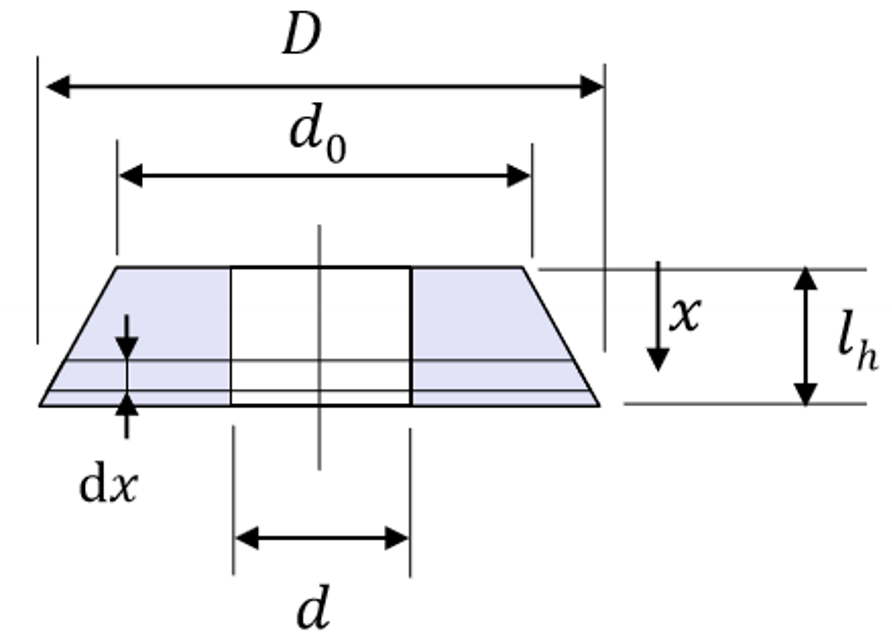
\includegraphics[width=4cm]{membstiff-det} \caption{} 
		\end{subfigure}
		\caption{cone of the altered stress distribution (a) and detailed representation of the cone with geometrical dimensions (b). } \label{fig:memberstiff}
	\end{figure}
	
	
	\paragraph{Pretension and interference} Considering that the members have a resting length of $l_{0f}$ while the bolts has length $l_{0b}$, it's then possible to compute the preload force $N_0$ that's acting between the components in order to ave a congruence between the equivalent springs (figure \ref{fig:preload}). The bolt elongates by a value $\Delta l_b$ while the member is tightened and so compressed by a value $\Delta l_f$; by analysing the problem the \textbf{tightening interference} $i_s$ between the components so became
	\begin{equation}
		i_s = \Delta l_b - \Delta l_f = N_0 \frac{K_f + K_b}{K_fK_b} \qquad \qquad \Rightarrow \qquad \Delta l_b = i_s \frac{K_f}{K_f + K_b} \qquad \Delta l_f = - i_s\frac{K_b}{K_f+K_b}
	\end{equation}
	To increase the preload it's sufficient to tighten more the bolt, decreasing so the resting length $l_{0b}$. In the case of \textbf{rigid members} (where so $K_f \gg K_b$) we can approximate $\Delta l_f$ to zero and $\Delta l_b = i_s$.
	
	Considering now to apply an extra separating load $N$ on the bolt, that's add an extra elongation $\Delta l$ on the threaded element, relieving the members and making them recovery some compression (figure \ref{fig:preload}.c). Graphically we can see how the force applied on the bolt increases to $N_b$ while the preload on the member decreases from $N_0$ to $N'$; in particular we have
	\begin{equation} \label{eq:boltloadpretension}
		N_b = N_0 + N \frac{K_b}{K_b+K_f} \hspace{3cm} N' = N_0 - N \frac{K_f}{K_b+K_f}
	\end{equation}
	
	
	\begin{figure}[bht]
		\centering
		\begin{subfigure}{0.325\linewidth}
			\centering 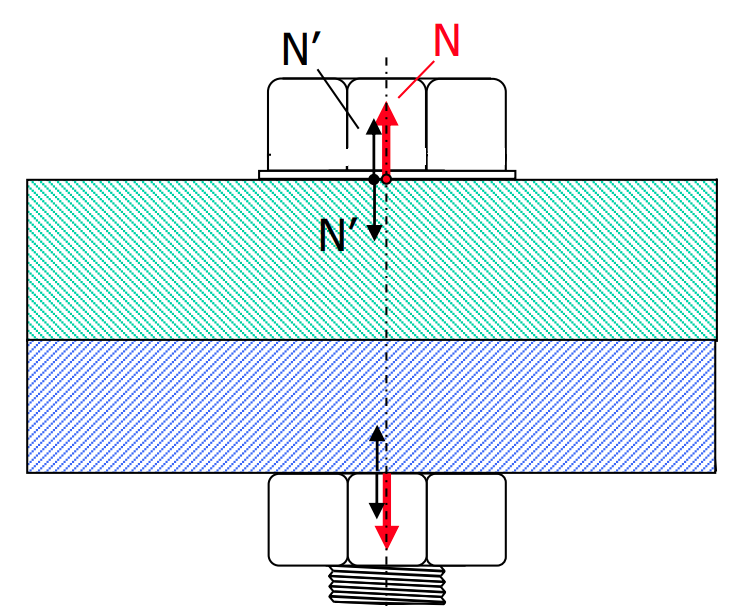
\includegraphics[width=4cm]{bolt-force} \caption{} 
		\end{subfigure}
		\begin{subfigure}{0.325\linewidth}
			\centering 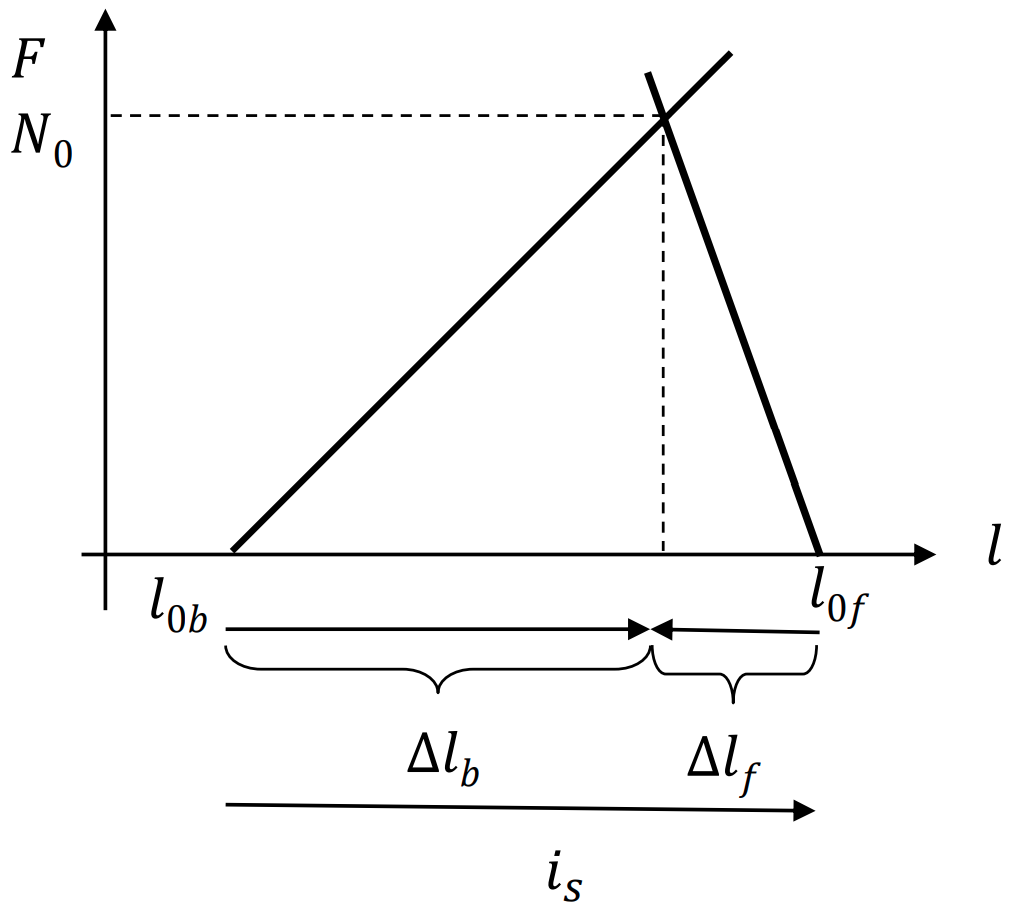
\includegraphics[width=5cm]{preload} \caption{} 
		\end{subfigure}
		\begin{subfigure}{0.325\linewidth}
			\centering 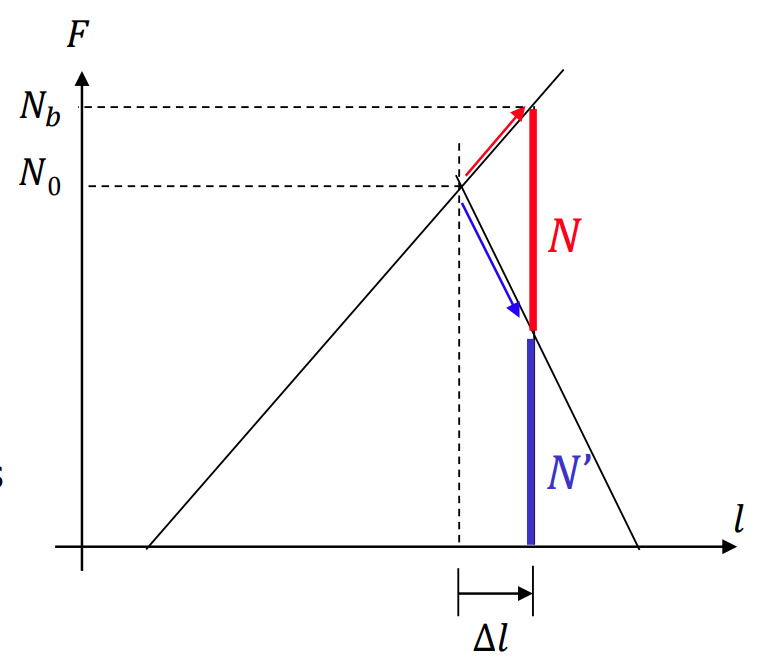
\includegraphics[width=5cm]{bolt-force-graph} \caption{} 
		\end{subfigure}
		\caption{forces exchanged between bolt and members (a), graph used to determine the preload force $N_0$ (b) and deformation due to more preload applied (c). } \label{fig:preload}
	\end{figure}
	
\subsection{Bolted joint analyses}
	The analyses of (multiple) bolted joints should be an hyper-static problem where however a simplified approach is taken into account to ease the solution.
\subsubsection*{Sliding actions}
	
	\paragraph{Shear} Considering the case of a connection that should bear a sliding load $V$ we assume that each bolt (having area $A_{b,i}$) bear a load parallel to the actual action and with module determined by the equation
	\begin{equation}
		V_i = V  \frac {A_{b,i}}{\sum_i A_{b,i}}
	\end{equation}
	This expression is made to make the system statically compatible, in fact $\sum_i V_i = V$.
	
	\paragraph{Torsion} Considering now the case of a connection that should bear a torque moment $T$ applied on the centroid $G$ of the section, we can define a relation similar to the previous one in order to determine a statically congruent system by determining that the shear loads $V_i$ on each bolts are 
	\begin{equation} \label{eq:slidetorsion}
		V_i = T \frac{A_{b,i}r_i}{\sum_i A_{b,i} r_i^2}
	\end{equation}
	where $r_i$ is the distance between the center of the bolt and the centroid $G$; $V_i$ is instead perpendicular to the radius vector $r_i$. To verify a bolted connection subject to shear load $V_i$ it's necessary to consider the friction coefficient $f$ between the connected members, and in particular we have to check that
	\begin{equation}
		V_i \leq f \frac{N'}{\phi} 
	\end{equation}
	where $\phi$ is the safety factor. By a static point of view we also need to check that
	\begin{equation} \label{eq:shearresistance}
		V_i \leq \frac{0.58 \suts A_{b,i}}{\phi}
	\end{equation}
	
\subsubsection*{Separating action}
	\paragraph{Normal load} Separating action happens every time the connection should bear normal loads within the members (and so connection subjected to normal load and bending). Considering the case of pure normal load $N$, similarly to the shear case, the action $N_i$ that each screw is subjected to evaluates as
	\begin{equation}
		N_i = N  \frac {A_{b,i}}{\sum_i A_{b,i}}
	\end{equation}
	In such case we have to verify that each bolt subjected to a normal action $N_{b,i} = N_0 + N_i \frac{K_b}{K_b+K_f}$ doesn't structurally fail with the common criteria of static analyses on beams. 
	
	
	
	\paragraph{Bending and normal loads} For normal and bending loads combined considering the simplified rigid members approach with bolts of equal cross section
	\[ N_i = \frac{M_b h_i}{\sum_i h_i^2} + \frac N{n_b} \]
	where $h_i$ can be measured from the more extremal pivot point of the section or (more conservative) at the first row of bolts. A more complex model is the semi-rigid approach where the load on each bolt is obtained by firstly solving the following system of differential equations in the variables $\sigma_{max,co}$ and $y_n$:
	\[ \left\{ \begin{aligned}
		& \int_0^{y_n} \sigma(y)\, dA + \sum_{i=1}^{n_{bt}} - \sigma_{max,co}\left(1-\frac{y_i}{y_n}\right)A_{b,i} = N \\
		& \int_0^{y_n} \big(y-y_n\big) \sigma(y)\, dA + \sum_{i=1}^{n_{bt}} - \sigma_{max,co}\left(1-\frac{y_i}{y_n}\right)\big(y_i-y_n\big)A_{b,i} = M_b 	+ N \big(y_g-y_n\big)
	\end{aligned} \right.   \]
	with $\sigma(y) = -\sigma_{max,co}\left(1-\frac{y_i}{y_n}\right)$ and $n_{bt}$ representing the number of bolts in tension; from the solution the load on each bolt is determined as
	\[ N_i = \sigma(y_i) A_{b,i} \]
	
\subsubsection*{Verification equation}
	To verify a bolted joint connection we must check:
	\begin{equation} \label{eq:boltverifications}
	\begin{aligned}
		\textrm{sliding:} \qquad & V \leq \frac{k_s n f}{\phi} N' = \frac{k_s,nf}\phi(N_0-N_e) \\
		\textrm{shear:} \qquad & V_b \leq \frac {A_b} \phi\suts && \textrm{eurocode 3: }\phi = \frac{1.25}{0.6}  \\
		\textrm{tension:} \qquad & N_b \leq \frac {A_{bt}} \phi \suts \qquad && \textrm{eurocode 3: }\phi = \frac{1.25}{0.9}  \\
		\textrm{crushing:} \qquad & V_b \leq \frac{dt}{\phi}\sigma_{uts,member} \\
		\textrm{punching:} \qquad & N_b \leq \frac{\pi d_0++ t}{\phi}\sigma_{uts,member}&& \textrm{eurocode 3: }\phi = \frac{1.25}{0.6}
	\end{aligned}
	\end{equation}
	where $d$ is the nominal diameter and $A_b = \pi 4 d^2$ the nominal area of the area; $A_{bt}$ the resisting cross-sectional area of the bolts, $d_0$ is the diameter of the bolt head diameter.
	
	Usually it's chosen
	\[ N_0 = 0.8 A_{bt}\sys \]
	
	
	
	
	
	
	
	
	
	
	
	
	
	
	
	
	
	
	
	
	